%%%% acra.tex

\typeout{ACRA Instructions for Authors}

% This is the instructions for authors for ACRA.
\documentclass{article}
\usepackage{acra}
\usepackage{lmodern}% http://ctan.org/pkg/lm
\usepackage{amsmath}
\usepackage{graphicx}
\usepackage{color}
\usepackage{hyperref}
\usepackage{amssymb}
\usepackage{url}
\usepackage{pdfpages}
\usepackage{fancyhdr}
\usepackage{subfig}
\usepackage{listings} 
\usepackage{selinput}    
\usepackage{tikz}
\newcommand{\quotes}[1]{``#1''}

% The file acra.sty is the style file for ACRA. 
% The file named.sty contains macros for named citations as produced 
% by named.bst.

% The preparation of these files was supported by Schlumberger Palo Alto
% Research, AT\&T Bell Laboratories, and Morgan Kaufmann Publishers.
% Shirley Jowell, of Morgan Kaufmann Publishers, and Peter F.
% Patel-Schneider, of AT\&T Bell Laboratories collaborated on their
% preparation. 

% These instructions can be modified and used in other conferences as long
% as credit to the authors and supporting agencies is retained, this notice
% is not changed, and further modification or reuse is not restricted.
% Neither Shirley Jowell nor Peter F. Patel-Schneider can be listed as
% contacts for providing assistance without their prior permission.

% To use for other conferences, change references to files and the
% conference appropriate and use other authors, contacts, publishers, and
% organizations.
% Also change the deadline and address for returning papers and the length and
% page charge instructions.
% Put where the files are available in the appropriate places.

\title{Fit a Gaussian Process}
\author{Diego Garrido}

\begin{document}

\maketitle
In this work we fit a Gaussian Process Regressor (GPR) with different kernel to different data set. \href{https://nbviewer.jupyter.org/github/dgarridoa/fit_gaussian_process/blob/main/Fit_Gaussian_Process.ipynb}{\color{blue}{Jupyter Notebook}}

\section{Fitting GPs over a sinusoidal function}

In this exercise we fit a Gaussian Process (GP) with different kernels to a sinusoidal function (see Figure 1). Based on fit on training set, the GP with the best performance, i.e., with higher likelihood, is the GP with Exponential Sine Squared (ESS) kernel, this has a log-likelihood of 3.394. However, GPs with kernels Radial Basic Funtion (RBF), Rational Quadratic (RQ) and Mattern kernel better capture smooth pattern of sinusoidal function. This can be seen by comparing the Root Mean Square Error (RMSE) in the intervale [0,5], where the RMSE of ESS is about twice the RMSE than the other kernels mentioned. Note that the RMSE is calculated by evaluating the sinusoidal function and the posterior mean on an equispaced sample of size 100 in the interval [0,5].\\
\begin{center}
\begin{figure}[!h]
    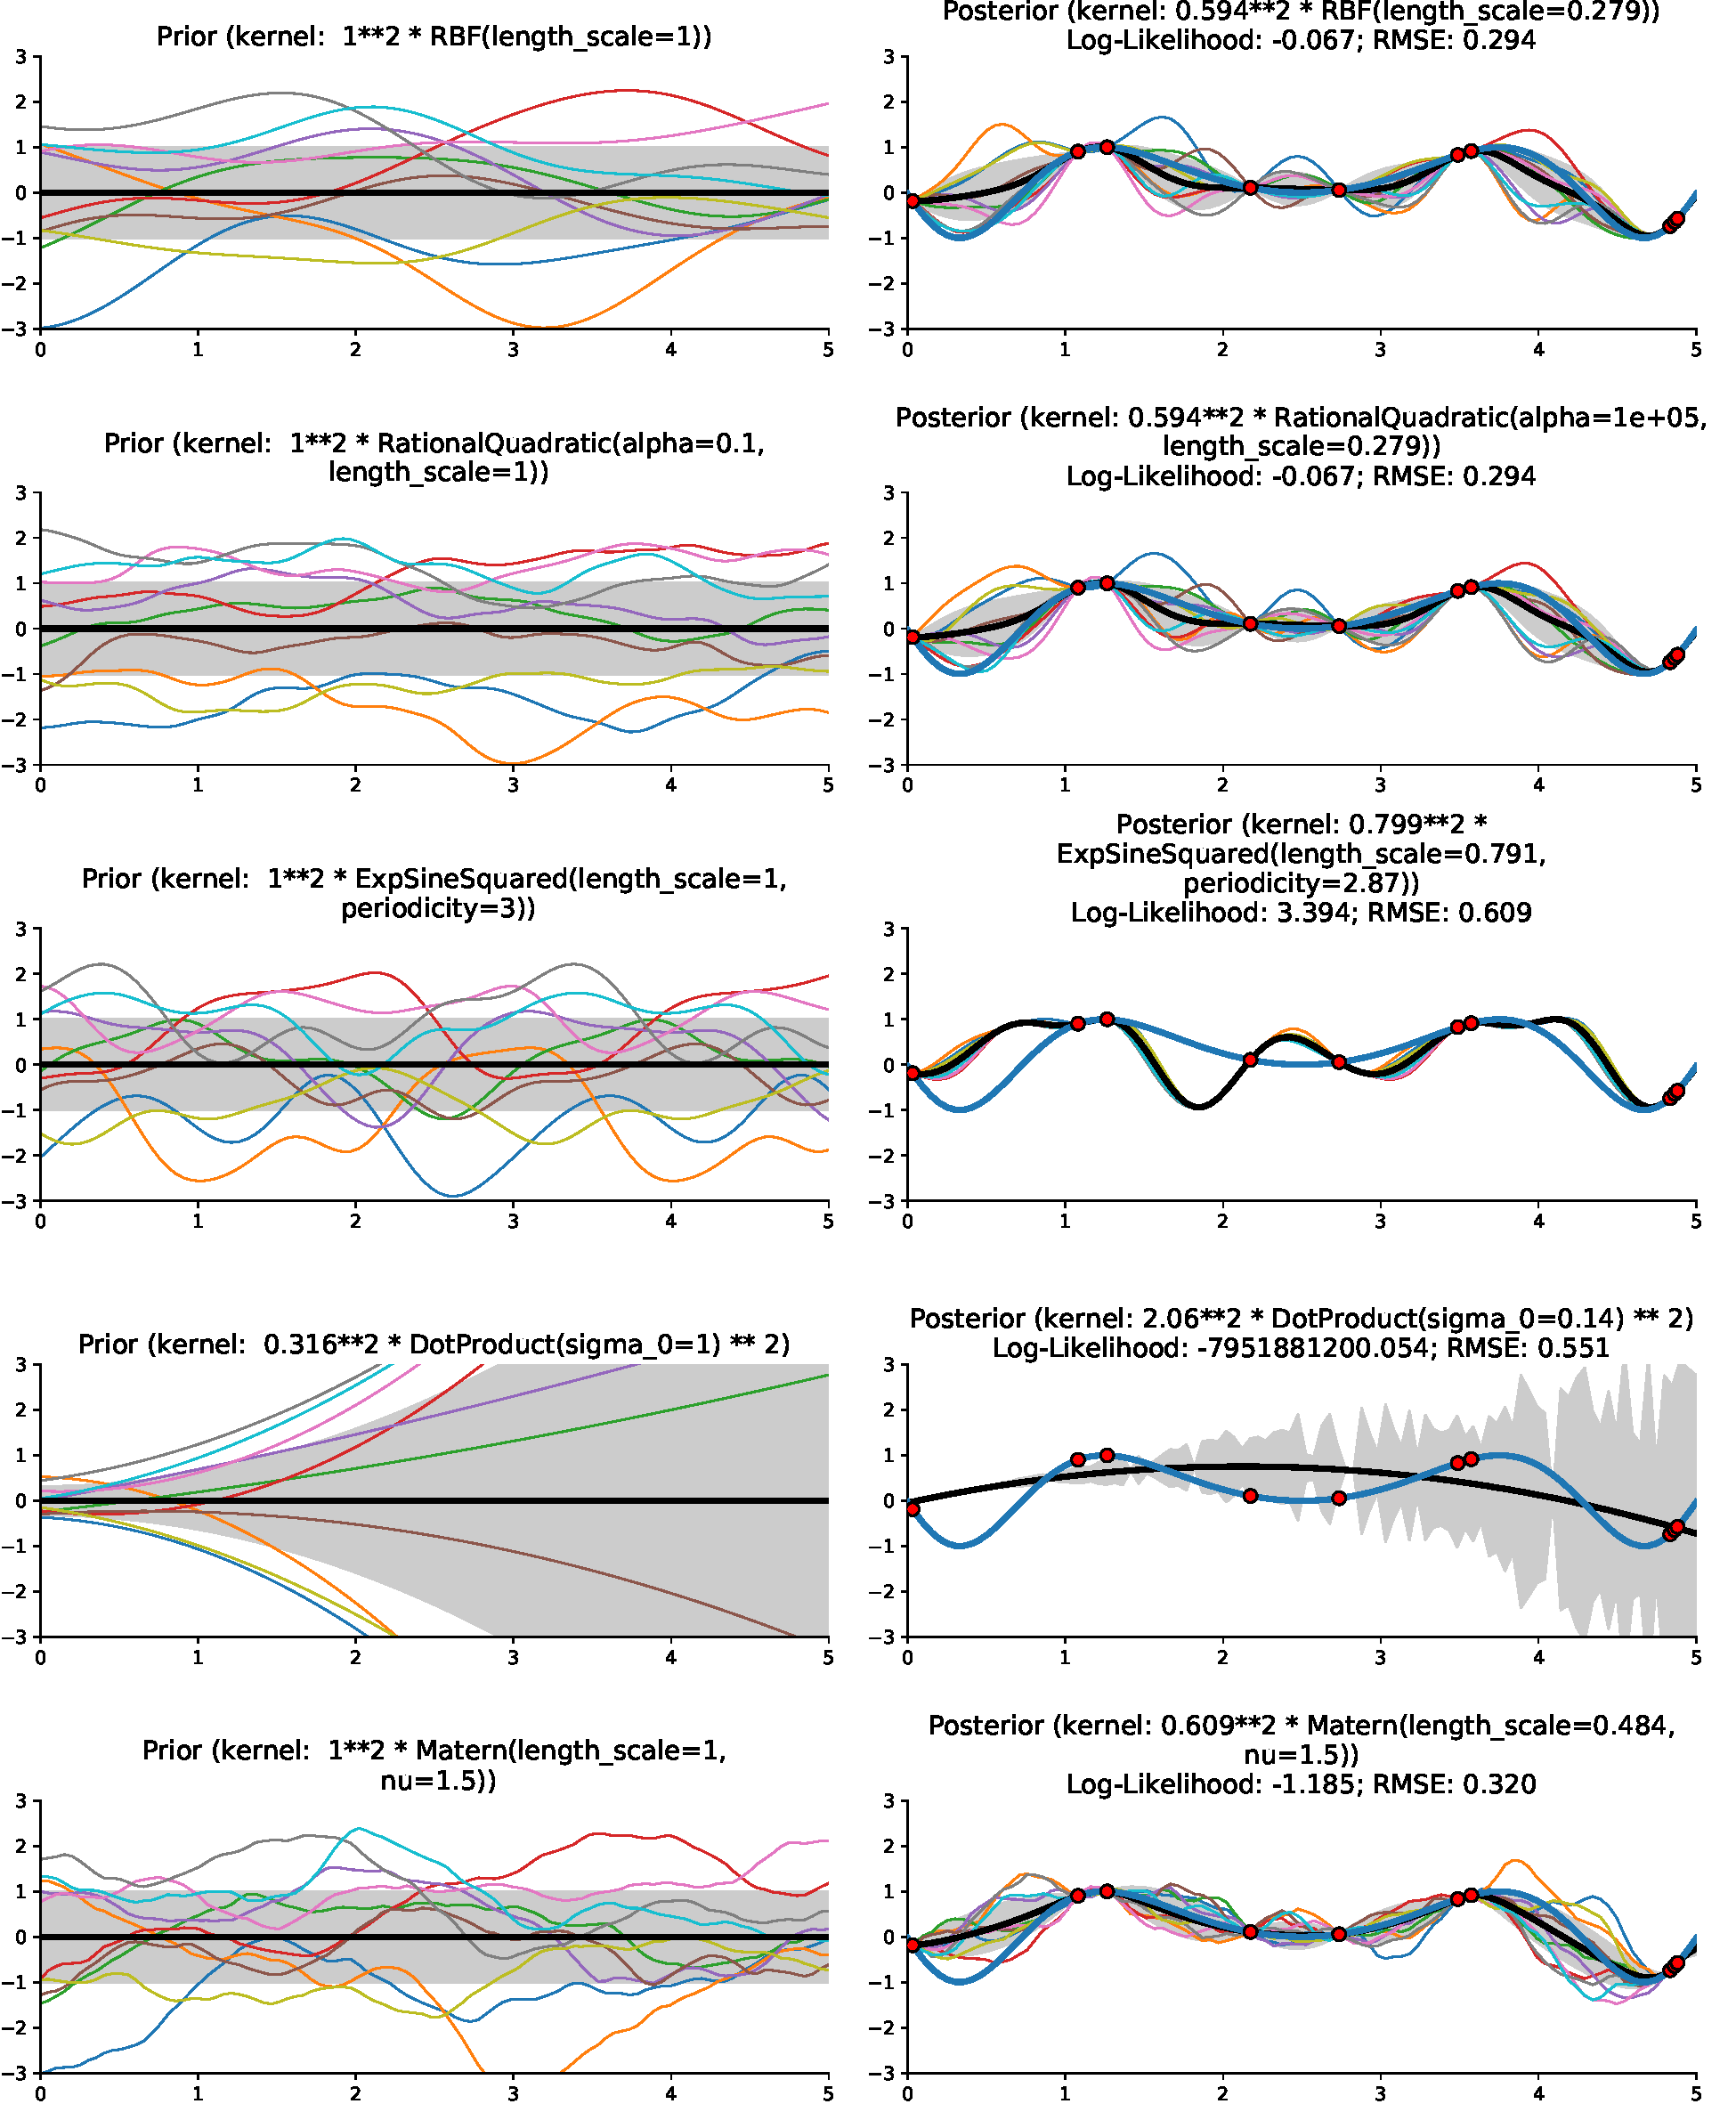
\includegraphics[width=0.5\textwidth]{img/gp1.pdf} 
    \caption{Prior and posterior of a Gaussian Process Regression with different kernels. Mean (black line), standard deviation (grey area), 10 samples (red points) and ground truth (blue line) are shown.}
\end{figure}
\end{center}
\section{Fitting GPs over a sample generated by a GP}

In this case, we generate 20 samples from a GP with RQ kernel and fit some GPs with different kernels (see Figure 2). Similarly, based on fit on training set, the GP with the best performance is the GP with monster kernel. This is because this kernel has great flexibility compared to the other kernels used. For that reason, this kernel is more likely to overfit data. To solve that problem, we can use a metric that penalize model complexity, such as the Bayesian Information Criteria (BIC), this metric penalizes the log-likelihood by the product between the number of free parameters $d$ (in this case, the parameters to be fitted) and the logarithm of the number of samples, mathematically is 

\begin{align}
    BIC = log p(D|\hat{\theta}_{ML})-\frac{d}{2}log(N)
\end{align}

, based in BIC the best model is the RQ kernel, the same one that generates the training data.

\begin{figure}[h]
    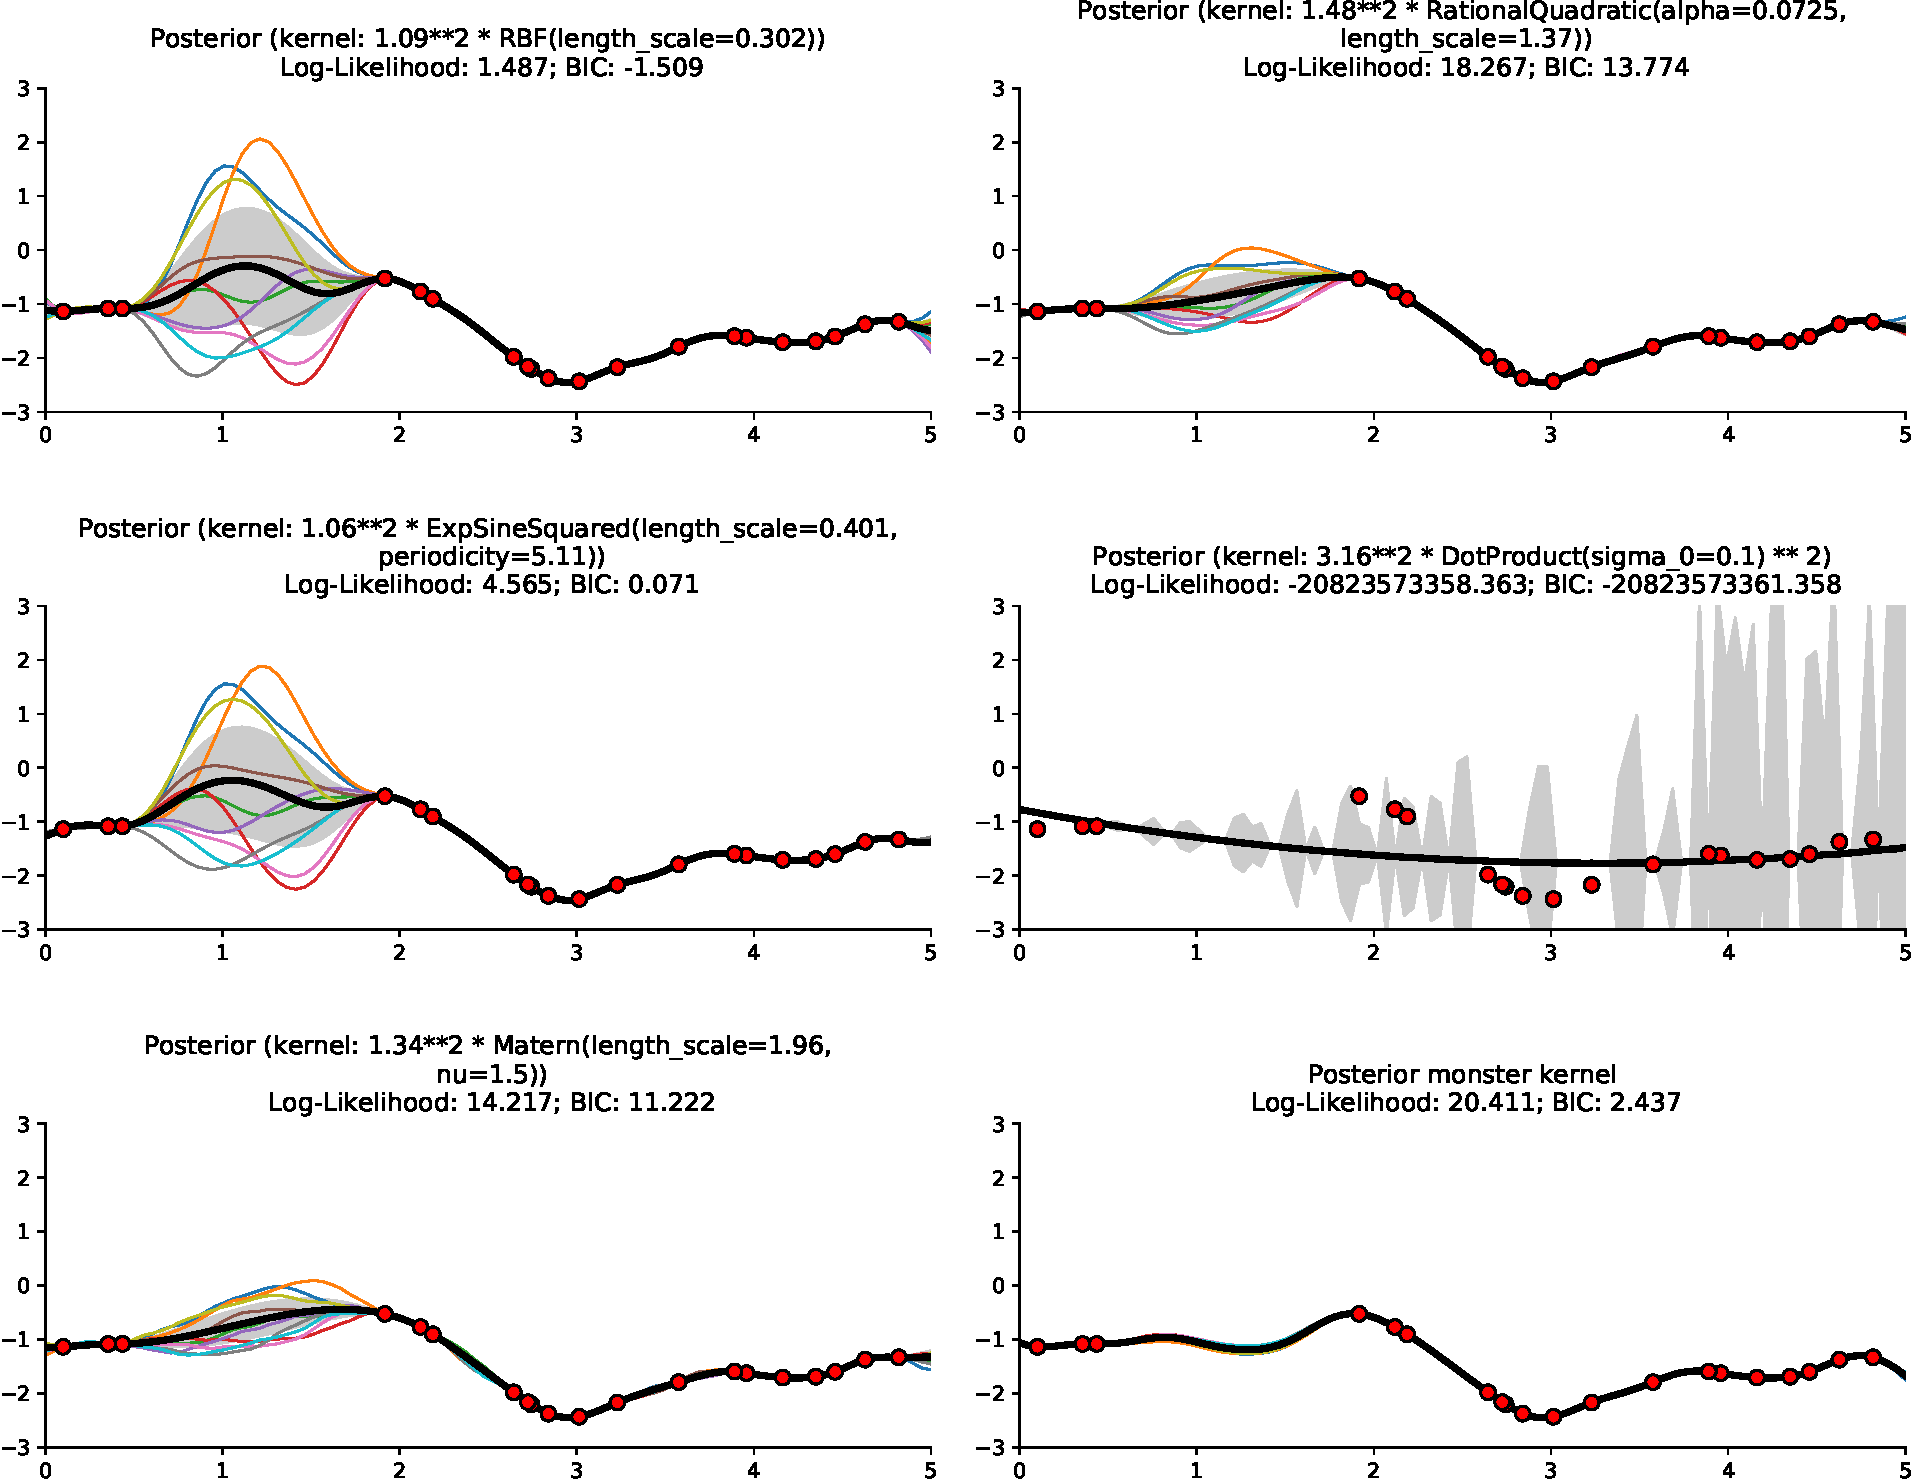
\includegraphics[width=0.5\textwidth]{img/gp2.pdf}  
    \caption{Posterior of a GPR with different kernels. Mean (black line), standard deviation (grey area) and 20 samples from a GP with RQ kernel (red points) are shown.}
\end{figure}

\section{Simplify kernel complexity}

When adjusting multiple kernels, a good heuristic to simplify the model is to start by eliminating those kernels that contribute less in magnitude, that is, the kernels with the lowest scale factor ($ \ sigma ^ {2} $). In this case for the monster kernel we have the follo parameters

\def\grayboxtext[#1,#2]#3{
        \node[fill=gray!80, text width=22em, draw=black!80, rounded corners, align=justify, below=#1] (#2) {#3}; 
}
\begin{figure}
\begin{tikzpicture}
    \grayboxtext[,t1]{\small Monster kernel parameters:
    0.669**2 * RBF(length\_scale=1.37) + 0.00316**2 * RationalQuadratic(alpha=1.33e+03, length\_scale=3.12) + 0.591**2 * ExpSineSquared(length\_scale=0.837, periodicity=2.93) + 0.1**2 * DotProduct(sigma\_0=1.8) ** 2 + 0.00316**2 * Matern(length\_scale=0.158, nu=1.5)};
\end{tikzpicture}
\caption{Monster kernel parameter from of a GPR fitted to 20 samples from a GP with RQ kernel.}
\end{figure}

, where we can see that scale factor ($\sigma^{2}$) from RQ and Matern are approximately five orders of magnitude lower than when used alone, and four orders less than RBF, ESS and Dot Product (DP).\\

\section{Increasing kernel complexity}

When kernels are added continuously the log-likelihood tends to increase (due to the increase in the complexity of the model), and by consequence the risk of overfitting too, this situacion is worse when we have small data or the phenomenon does not have high complexity. This problem can be solved evaluating the generalization capacity in validation set (not seen on training time) from differents kernels, using metric like RMSE or Mean Absolute Error (MAE), since it is a regression problem. Alternatively, we can use information theory metrics such as BUC or Akaike Information Criteria (AIC), these measure penalize the log-likelihood by model complexity, in this way, a more complex model requires an increase in performance according to the increase in complexity.\\

\section{Setting the init kernel parameter in a GP}

We create a synthetic signal, where the training data $D = \{x_{i},y_{i}\}_{i=1}^{10}$, the $x_{i}$ are i.i.d as a $U(0,5)$ and $y_{i} = x_{i}+cos(2\pi x_{i})$ (see Figure 4). How the data look non-stationary and periodic we use a DP plus ESS kernel, this is illustrated in equations 2-4. 

\begin{align}
k_{DP}(x,x') &= \sigma_{0}^{2}+x_{i}x_{j}\\
k_{ESS}(x,x') &= exp\bigg(\frac{2sin^{2}(\pi |x-x'|/p)}{l^{2}}\bigg)\\
k(x,x') &= \sigma_{DP}^{2}k_{DP}(x,x')+\sigma_{ESS}^{2}k_{ESS}(x,x')
\end{align}

The objective function of a GP is not convex, this is why it becomes very important to choose the initial parameters correctly to start near a good local optimum. The init parameters for the $k_{DP}$  were chosen using a linear regression. The linear regression was fitted on training data, with $\theta_{0}$ as intercept and $\theta_{1}$ as slope. Then the setting was $\sigma_{DP}^{2}$ equal to the slope and $\sigma_{0}^{2}$ equal to the intercept. The variance with respect to the mean estimated by the linear regression is used as $\sigma_{ESS}^{2}$, i.e., $\sigma_{ESS}^{2}=\frac{\sum_{i=1}^{N}(\theta_{0}+\theta_{1}x_{i}-y_{i})^{2}}{N}$. The periodicity $p$ was setted in 1 with bound between [1,10], this is due that in the interval [0,5] we has 10 samples, so the maximum peridiocity that we can observe is 10 (twice the interval size) and the minimum is 1 (twice the interval size divided by the number of samples). Finally, the $\ell$ parameter controls the smoothness, as this is not much, it was set to a value of 1 with a limit of [0.1,10].

\begin{figure}[h]
    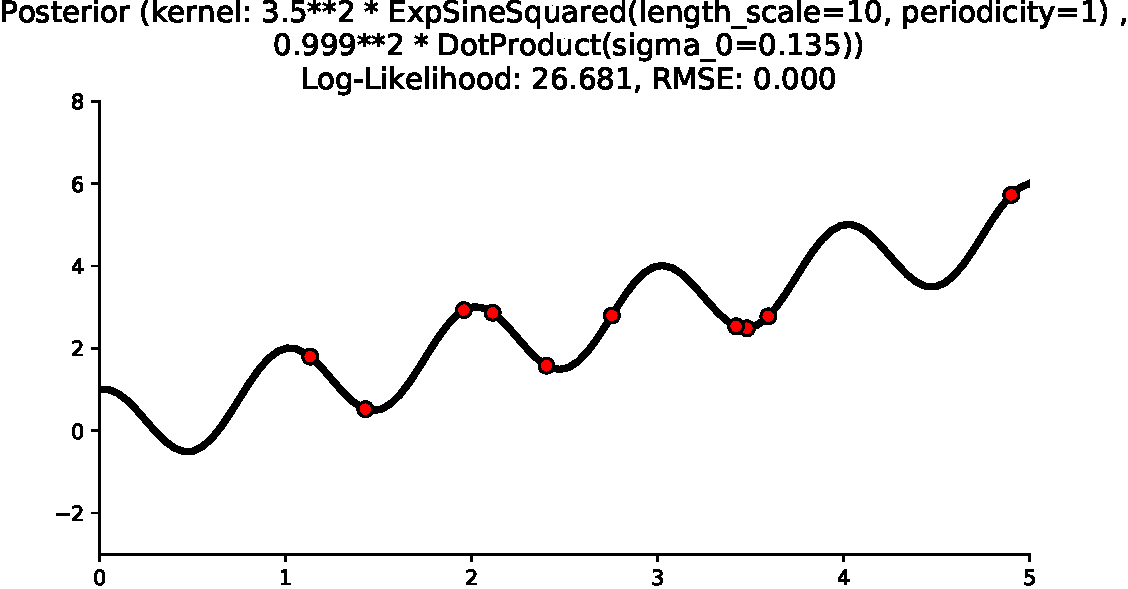
\includegraphics[width=0.5\textwidth]{img/gp3.pdf}
    \caption{Posterior of a GPR with kernel DP plus ESS. Mean (black line) and 10 samples (red point).}
\end{figure}


\end{document}